\documentclass[12pt]{report}

\usepackage{geometry}
\geometry{a4paper,scale=0.8}

\usepackage{indentfirst}
\usepackage{caption}
\usepackage{graphicx, subfig}

\usepackage[BoldFont,SlantFont,CJKchecksingle]{xeCJK}
\setCJKmainfont[BoldFont=SimHei,SlantedFont=KaiTi]{SimSun}
\setCJKsansfont[BoldFont=SimHei,SlantedFont=KaiTi]{SimSun}
\setCJKmonofont[ItalicFont={Adobe Fangsong Std}]{SimSun}
\setCJKfamilyfont{zhsong}{SimSun}
\newcommand{\song}{\CJKfamily{zhsong}} 
\setCJKfamilyfont{zhhei}{SimHei}
\newcommand{\hei}{\CJKfamily{zhhei}}
\setCJKfamilyfont{zhkai}{KaiTi}
\setCJKfamilyfont{zhfs}{FangSong}
\newcommand{\xiaoyihao}{\fontsize{24pt}{\baselineskip}\selectfont}      %小一号  
\newcommand{\erhao}{\fontsize{21pt}{\baselineskip}\selectfont}      %二号  
\newcommand{\xiaoerhao}{\fontsize{18pt}{\baselineskip}\selectfont}  %小二号  
\newcommand{\sanhao}{\fontsize{15.75pt}{\baselineskip}\selectfont}  %三号  
\newcommand{\sihao}{\fontsize{14pt}{\baselineskip}\selectfont}%     四号  
\newcommand{\xiaosihao}{\fontsize{12pt}{\baselineskip}\selectfont}  %小四号  
\linespread{1.2}
\setcounter{secnumdepth}{3}
\setcounter{tocdepth}{3}

\title{生态系统网络}

\author{姓名:庞冰瑶\\
	    学号:21721127}


\date{}

\begin{document}
   
	\begin{center}
		\vspace*{8mm}
		\hei\xiaoyihao\textbf{生态系统网络}\\
	\end{center}
	
	\vspace{7cm}
	
	\begin{tabbing}       %tabbing  列表
		
		\hspace*{5cm} \= \hspace{3cm} \= \kill  
		% \=     in tabbing environment, sets a tab stop
		% \kill  in a\tabbing environment, deletes previous line so tabs can be set without outputting text.
		% \>     in tabbing environment is a forward tab.
		% 这次的居中 用的 \centering  ,注意三次的区别。
		\>{\song\sihao\textbf {姓\hspace{0.5cm}名\ \ :}} \> 
		{\centering\song\sihao\textbf{~~~~~~~~庞冰瑶~~~~~~~~~~~}}\\ 
		% 总长3.4cm
		\\
		\>{\song\sihao\textbf {学\hspace{0.5cm}号 \ \ :}}\>  {\centering\song\sihao\textbf{~~~~~~21721127~~~~~~~~~}} \\
		 
   \end{tabbing}	
	\tableofcontents	
	\renewcommand\thesection{\arabic {section}}
	\newpage
	\section{复杂网络}
	\subsection{复杂网络}
	
 复杂网络是具有自组织、自相似、吸引子、小世界、无标度中部分或全部性质的网络。其具有如下特性:
	\par\setlength\parindent{2em}第一,小世界。即大多数网络尽管规模很大,但是任意两个节(顶)点间却有一条相当短的路径。例如,在社会网络中,人与人相互认识的关系很少,但是却可以找到很远的无关系的其他人。
	\par\setlength\parindent{2em}第二,集群即集聚程度。例如,社会网络中总是存在熟人圈或朋友圈,其中每个成员都认识其他成员。集聚程度的意义是网络集团化的程度;这是一种网络的内聚倾向。连通集团概念反映的是一个大网络中各集聚的小网络分布和相互联系的状况。例如,它可以反映这个朋友圈与另一个朋友圈的相互关系。
	\par\setlength\parindent{2em}第三,幂律的度分布概念。度指的是网络中顶(节)点(相当于一个个体)与顶点关系(用网络中的边表达)的数量;度的相关性指顶点之间关系的联系紧密性;介数是一个重要的全局几何量。顶点u的介数含义为网络中所有的最短路径之中,经过u的数量。它反映了顶点u(即网络中有关联的个体)的影响力。无标度网络的特征主要集中反映了集聚的集中性。
	
	
	\subsection{生态系统网络}
	生态网络是对生态系统中物质、能量流动进行模拟的结构模型。生态网络分析是指对生态网络进行分析的方法和理论。它在年代后期开始引起人们的注意。其领域涉及生态网络流动分析、信息分析、随机分析、结构分析以及灵敏度分析等。它是系统生态学的重要分支。其中传染病模型是其中的重要模型。
	\begin{figure}
		\centering
		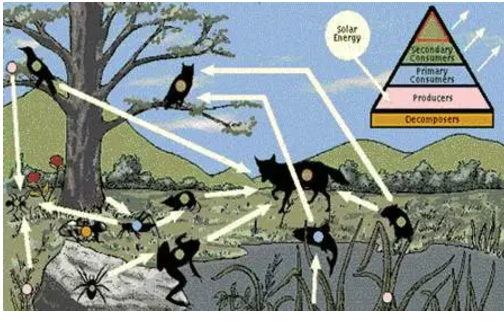
\includegraphics[width=0.8\textwidth]{img/stnetwork.png}
		\caption{生态系统网络} 
		\label{img}
	\end{figure}
	\section{基本传染病模型}
	
	
	\subsection{研究意义}
	
	传染病是影响人们身体健康的重要因素之一,长期以来受到世界各国的关注。人员的频繁交流和接触、全球环境污染日趋恶化等加剧了传染病在全球范围的传播。原来已几乎灭绝和被控制的某些传染病再次抬头并有蔓延的趋势。一些新出现的传染病来势凶猛,例如, 2003年春季在我国及周边国家爆发的大规模的“非典型性肺炎”(简称SARS) ,严重地危害了人类的健康。因此研究传染病的传播过程、内在规律及其如何采取控制措施具有重要意义。
	
	\subsection{基本的传染病模型}
	
	在一般的传染病传播过程中人口总数可以近似看作常量(传染病传播时间比较短,例如3到5个月,在短时间内,人口总数变化很小,即不考虑出生、死亡和人口迁移);人群均匀分布,人群中的个体没有差异。在这个基础下,有三种基本的传染病模型:SI,SIS,SIR。
	
	\setcounter{secnumdepth}{3}\subsubsection{SI模型}
	SI模型不考虑病人的治愈,只考虑健康者被感染成为病人。
	\par\setlength\parindent{2em}假设,每个病人每天可使$\lambda s(t)$个健康者变为患者,病人数为$Ni(t)$,所以每天共有$\lambda Ns(t)i(t)$个健康者被感染,于是$\lambda Nsi$就是病人数$Ni$的增加率,即
	$N di/dt=\lambda Nsi$
	又因为
	$s(t)+i(t)=1$
	
	初试时刻(t=0)病人比例为$i_0$,则
	$$di/dt=λi(1-i),i=i_0$$
	
	上式解为
	$$i(t)=1/(1+(1/i_0 -1)e^{-\lambda t} )$$
	
	在该模型中,当t→∞时i→1,即所有人均被感染,如图2,这明显不符合现实。原因是,模型没有考虑病人会痊愈。
	
	
	\begin{figure}
		\centering
		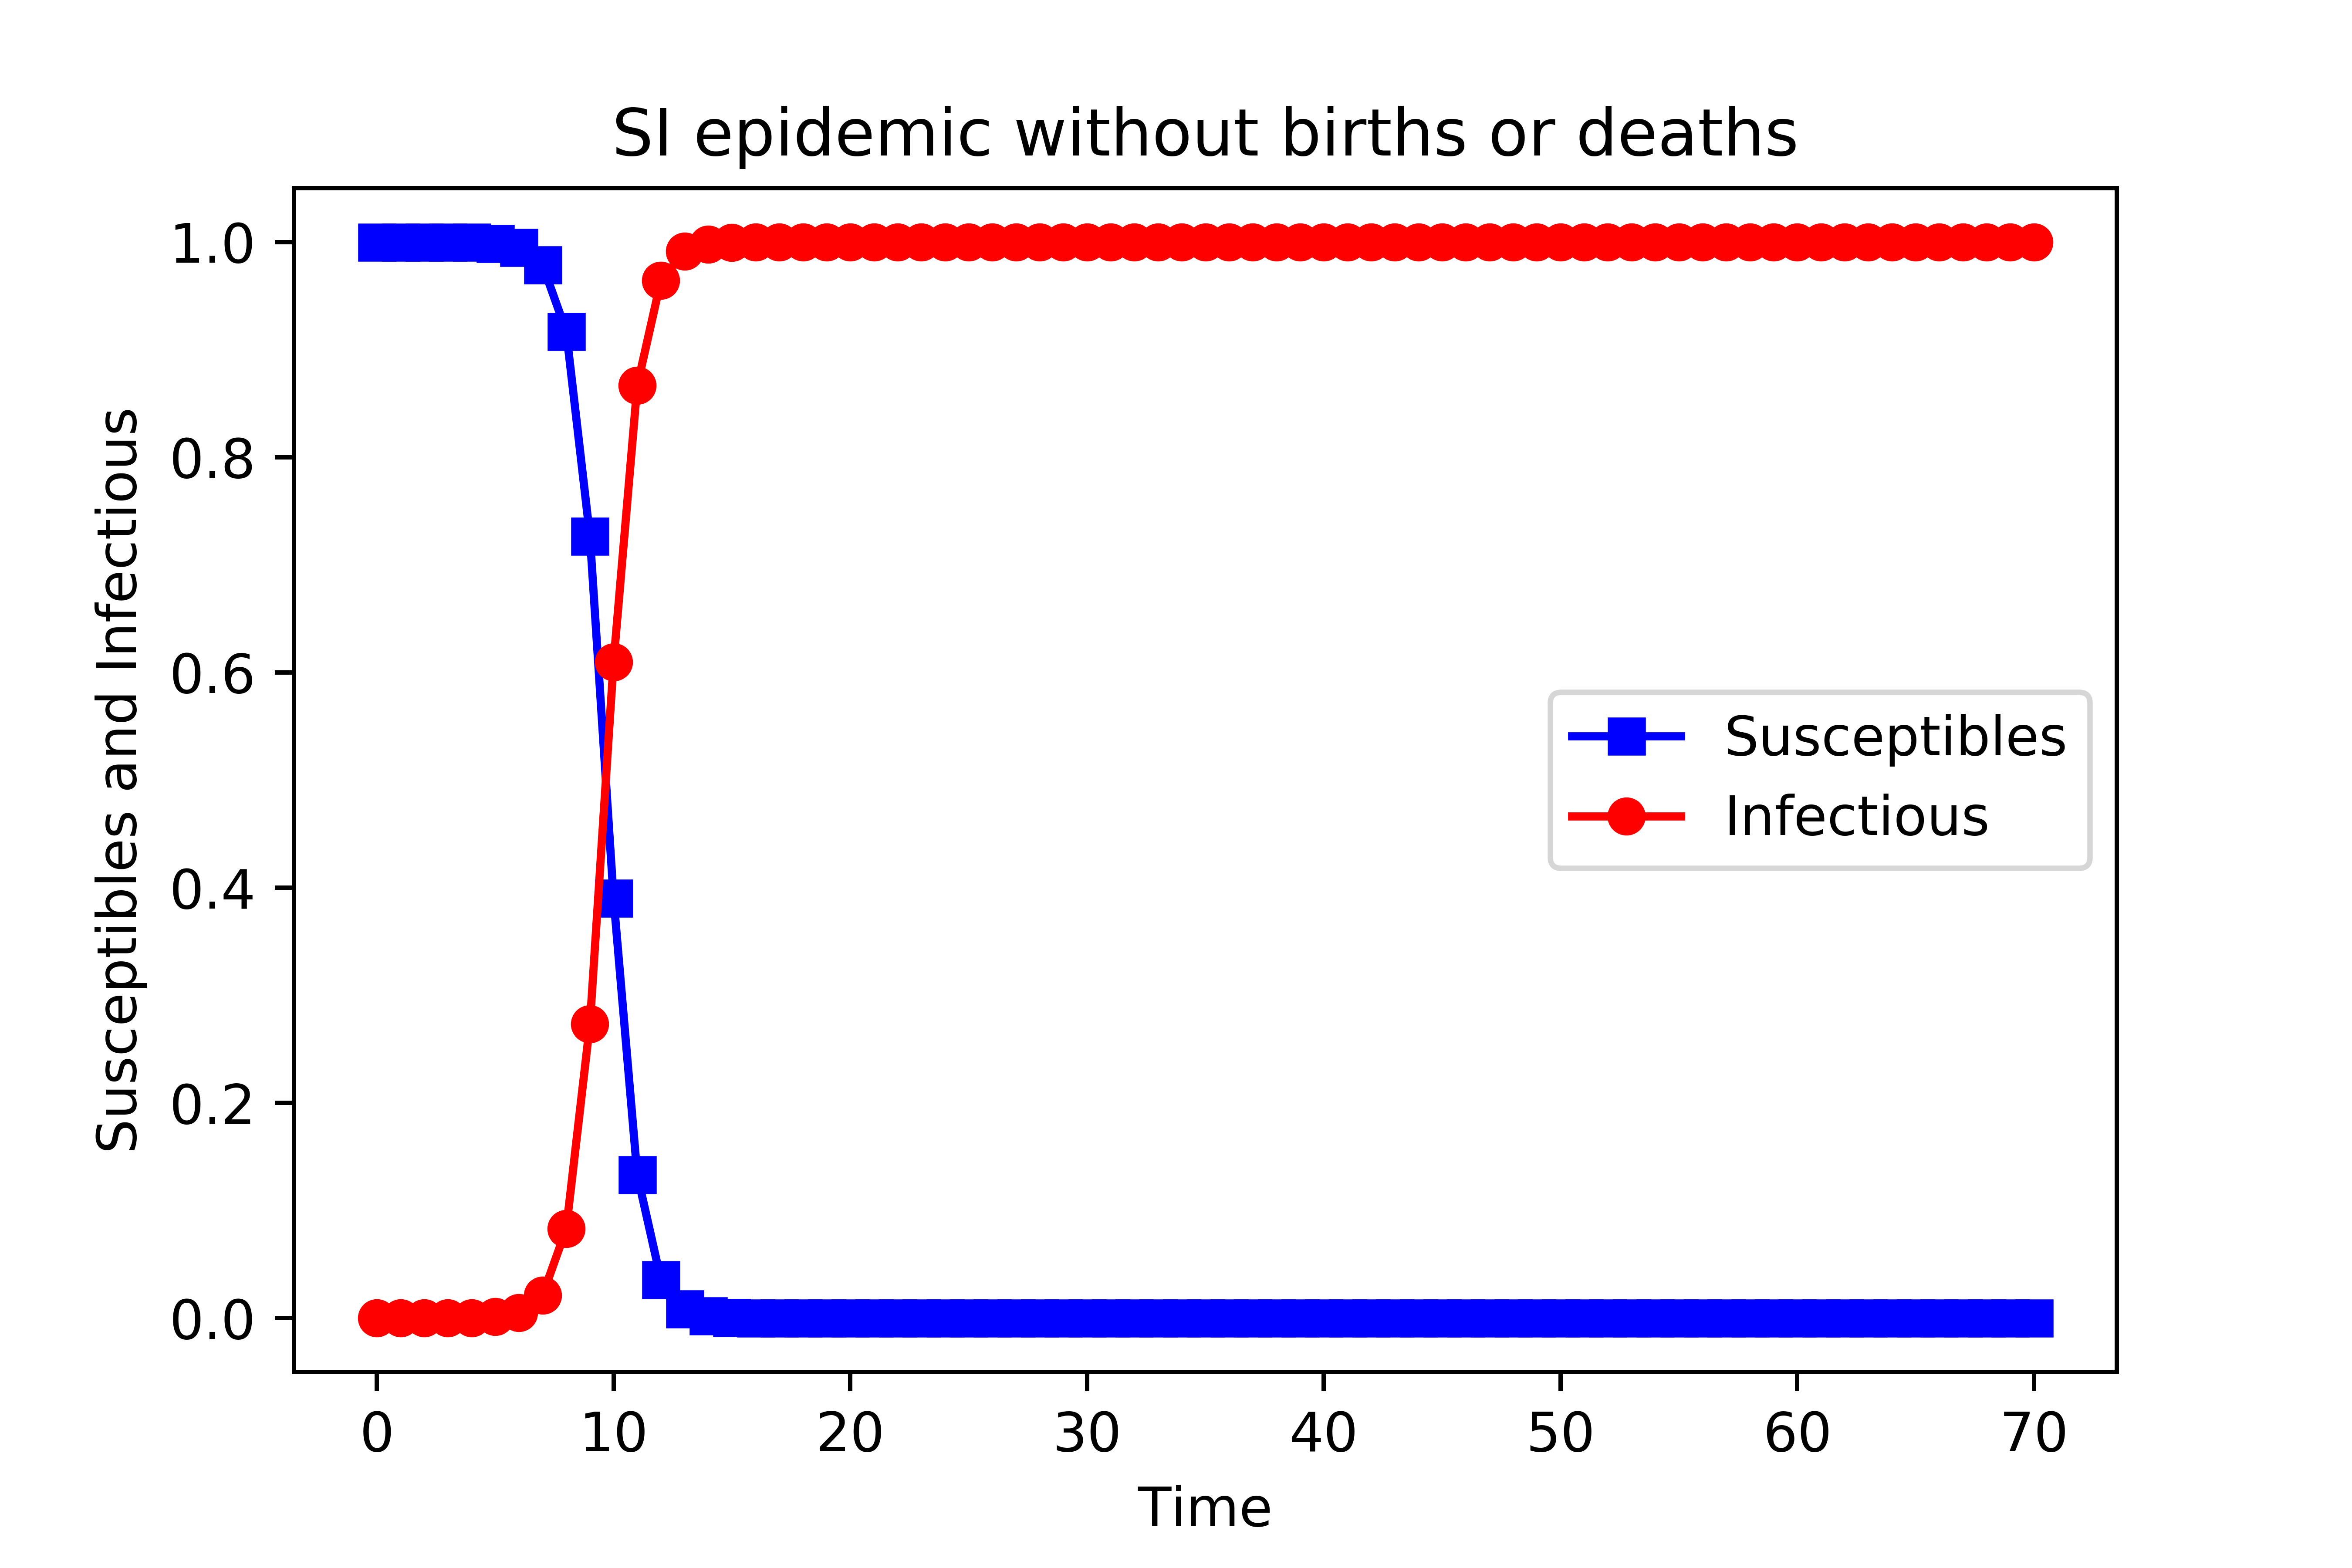
\includegraphics[width=0.8\textwidth]{img/SI.png}
		\caption{SI} 
		\label{img}
	\end{figure}
	\setcounter{secnumdepth}{3}\subsubsection{SIS模型}
	SIS模型为病人被治愈后变成健康者,健康者还可以被感染变成病人。例如有些传染病如伤风、痢疾等愈合后免疫力很低,假定无免疫力。起初你容易感染某一种疾病并确实被感染,得到治疗并痊愈,但是你会再一次面临被传染的风险。于是:
	$$N[i(t+\delta t)-i(t)]=\lambda Ns(t)i(t)\delta t-\mu Ni(t)$$
	
	则微分方式为:
	$$di/dt=\lambda i(1-i)-\mu i,i=i_0$$
	
	定义$\sigma=\lambda ⁄\mu$,其中,$\sigma$是整个传染期间内每个病人有效接触的平均人数,称为接触数。
	$$di/dt=-\lambda i[i-(1-1/\sigma)],i=i_0$$

   由于个体被感染后可以恢复,所以在一个时间点上,系统会到达稳态,图3中是t=17,系统达到一个稳态,其中感染个体的比例是恒定的。因此,在稳定状态下,只有有限部分的个体被感染,此时并不意味着感染消失了,而是此时在任意一个时间点,被感染的个体数量和恢复的个体数量达到一个动态平衡,双方比例保持不变。
	
	\begin{figure}
		\centering
		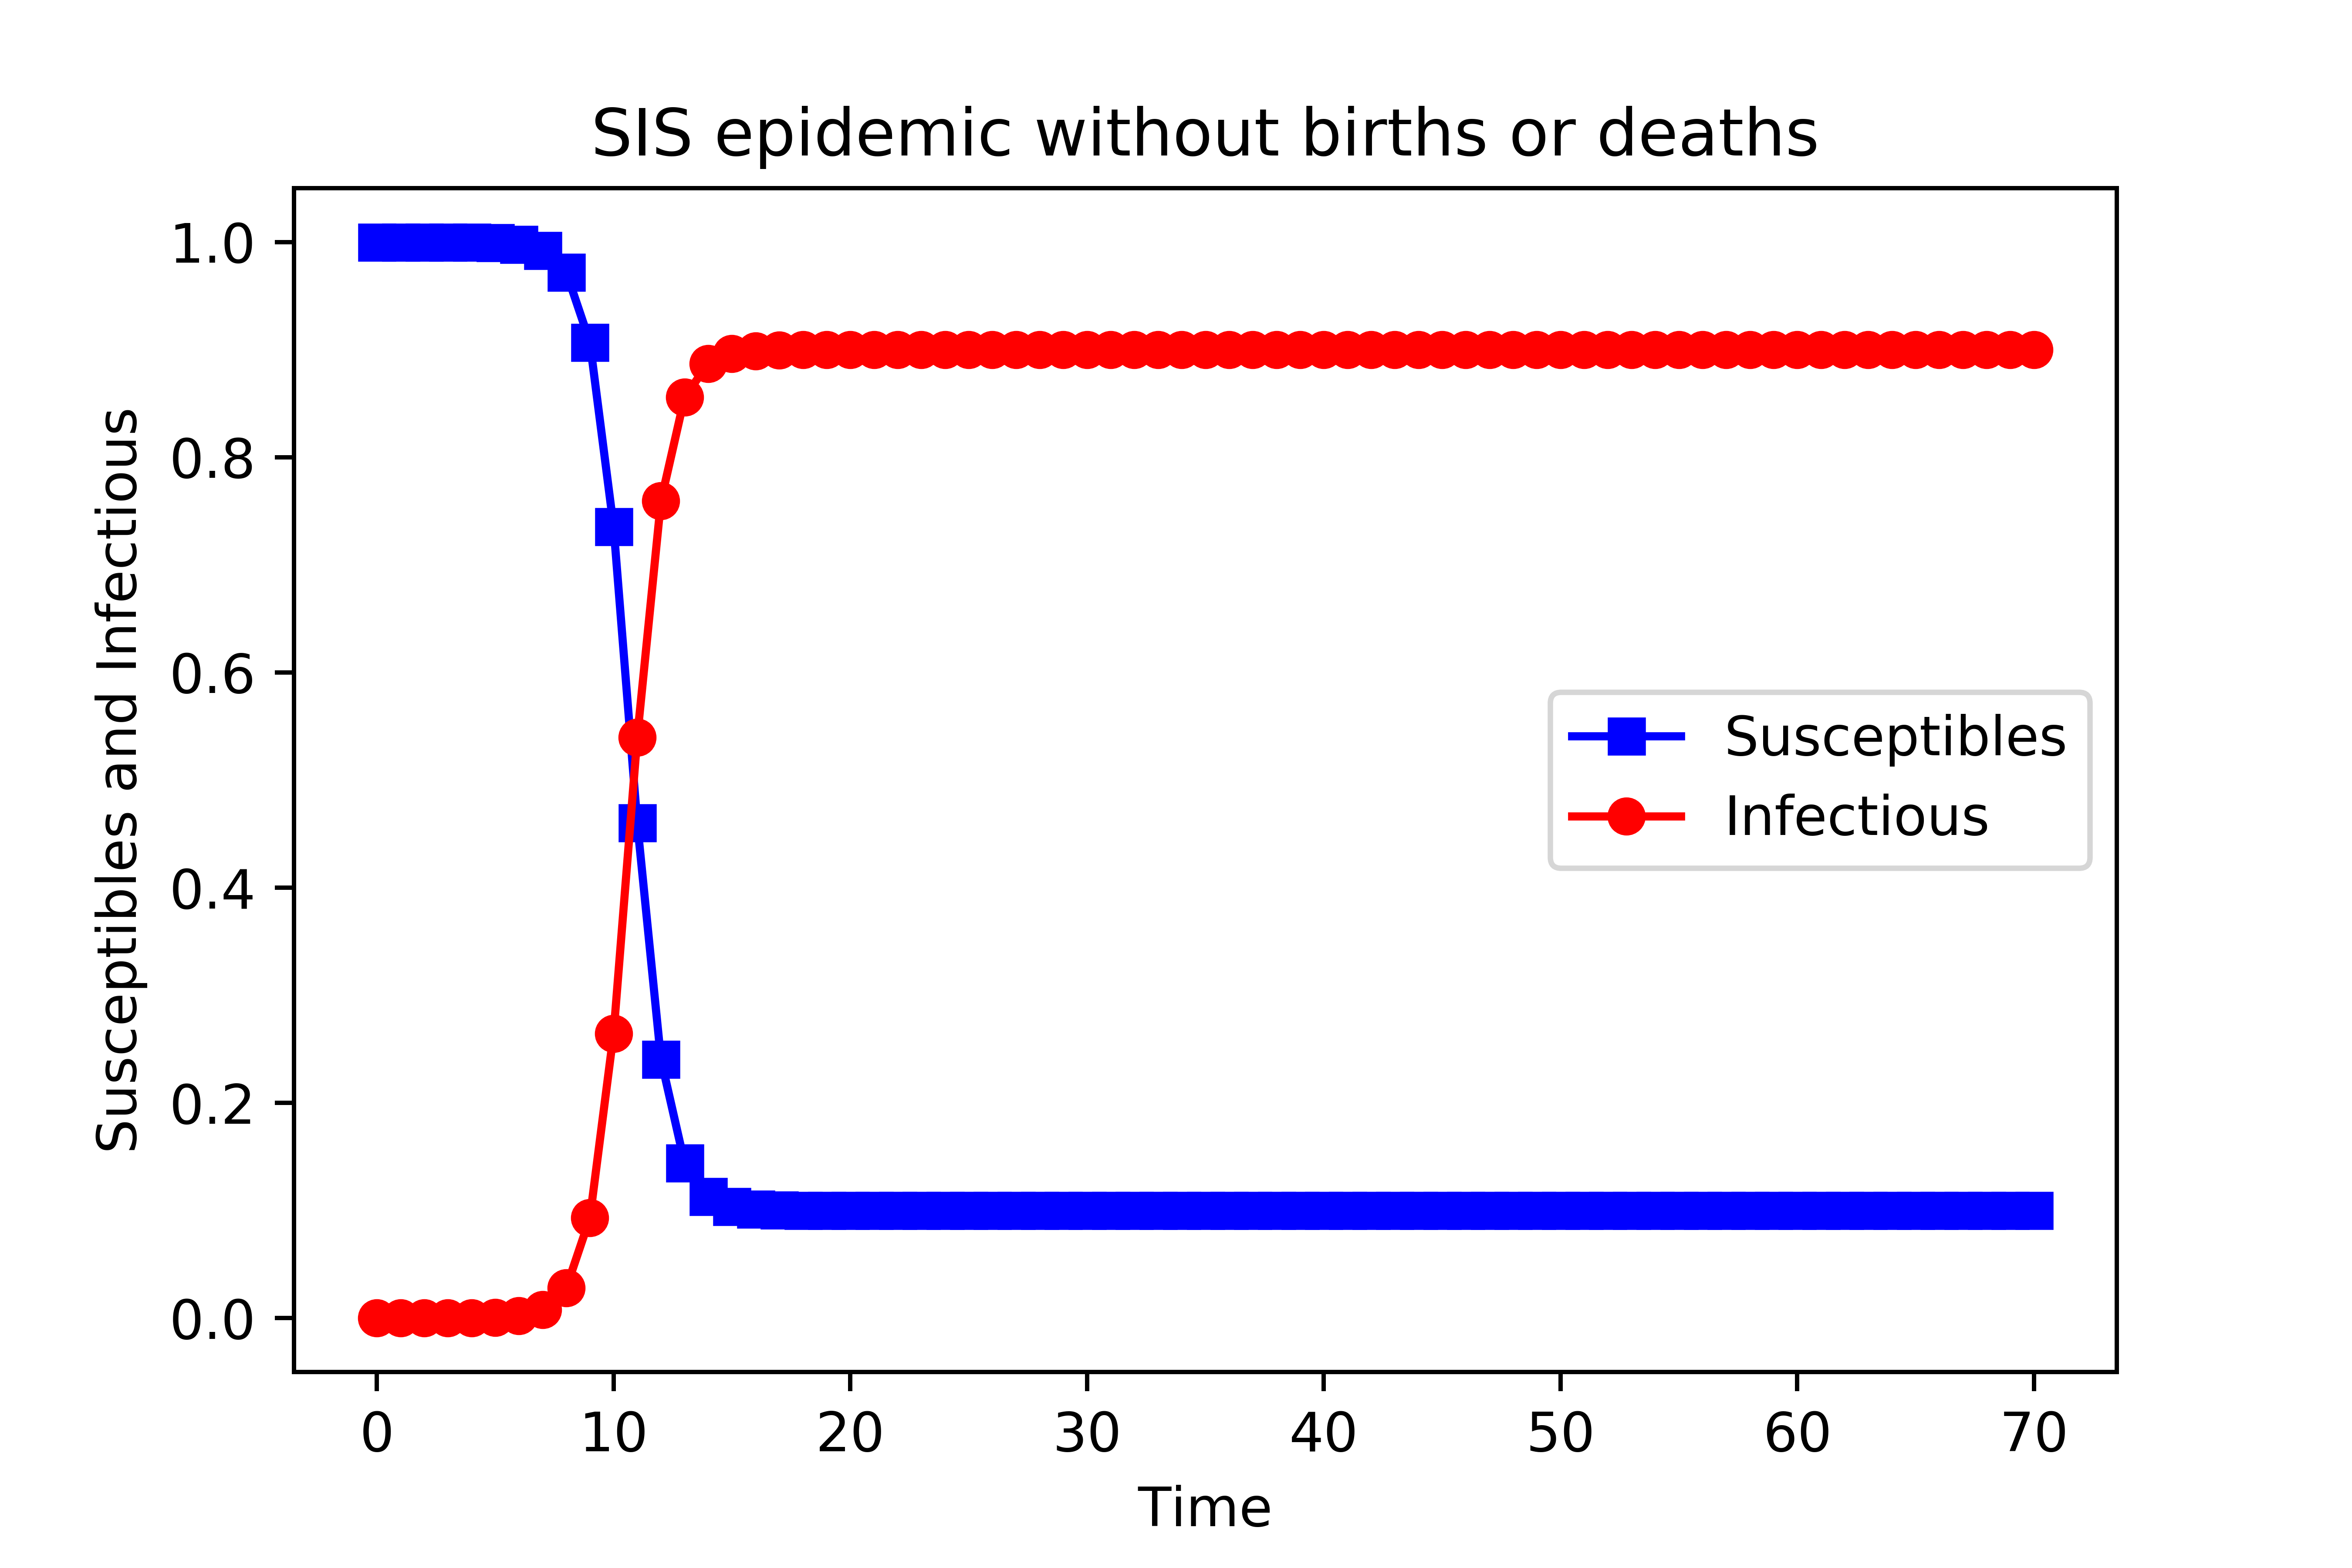
\includegraphics[width=0.8\textwidth]{img/SIS.png}
		\caption{SIS} 
		\label{img}
	\end{figure}
	\setcounter{secnumdepth}{3}\subsubsection{SIR模型}
	
	SIR模型是指易感染者被传染后变为感染者,感病者可以被治愈,并会产生免疫力,变为移除者(R)。适用于那些使传染者感染后可以得到免疫力的例子。健康人被感染之后被治愈,然后会对这种疾病产生抗性并不会再被感染。人员流动为S-I-R形式。
	\par\setlength\parindent{2em}则在SIR模型中有$s(t)+i(t)+r(t)=1$。对于病愈的免疫移除者的数量应满足如下公式:
	$$N dr/dt=\mu Ni$$
	
	设初始时刻,易感者、传染病者、恢复者的比例分别为$s_0 (s_0>0)$,$i_0 (i_0>0)$,$r_0=0$,则微分方程如下:
	$$di/dt=\lambda si-\mu i$$
	$$ds/dt=-\lambda si$$
	$$r/dt=\mu i$$

   通常人们认为仅当病人比例有一段增长时才认为传染病在蔓延,而1 / a 是一个非常关键的量, 根据该量可得到以下两种控制传染病的蔓延方法。
   \par\setlength\parindent{2em}一种方法是当$s_0>l/\sigma$时传染病蔓延, 我们只要想办法提高$l/\sigma$, 的值使得$s_0<=l/\sigma$, 传染病就不会蔓延(初始时期的健康者的比例是定值$s_0\approx l/\sigma$ )。又因为人们的卫生水平越高$\lambda$越小,医疗水平越高$\mu$越大,于是$l/\sigma$越大,故提高卫生水平和医疗水平有助于控制传染病的蔓延。
   \par\setlength\parindent{2em}另一种方法是当$s_0>l/\sigma$时, 在人们的卫生水平和医疗水平不改变的条下,降低初始人群中健康者的比例$s_0$使得$s_0<=l/\sigma$,传染病也不会蔓延。要降低$s_0$,必须提高传染病的治愈人数和免疫人数。这就要求我们在发展免疫方面提高免疫能力,同时努力提高传染病的治愈率。
		
		\begin{figure}
			\centering
			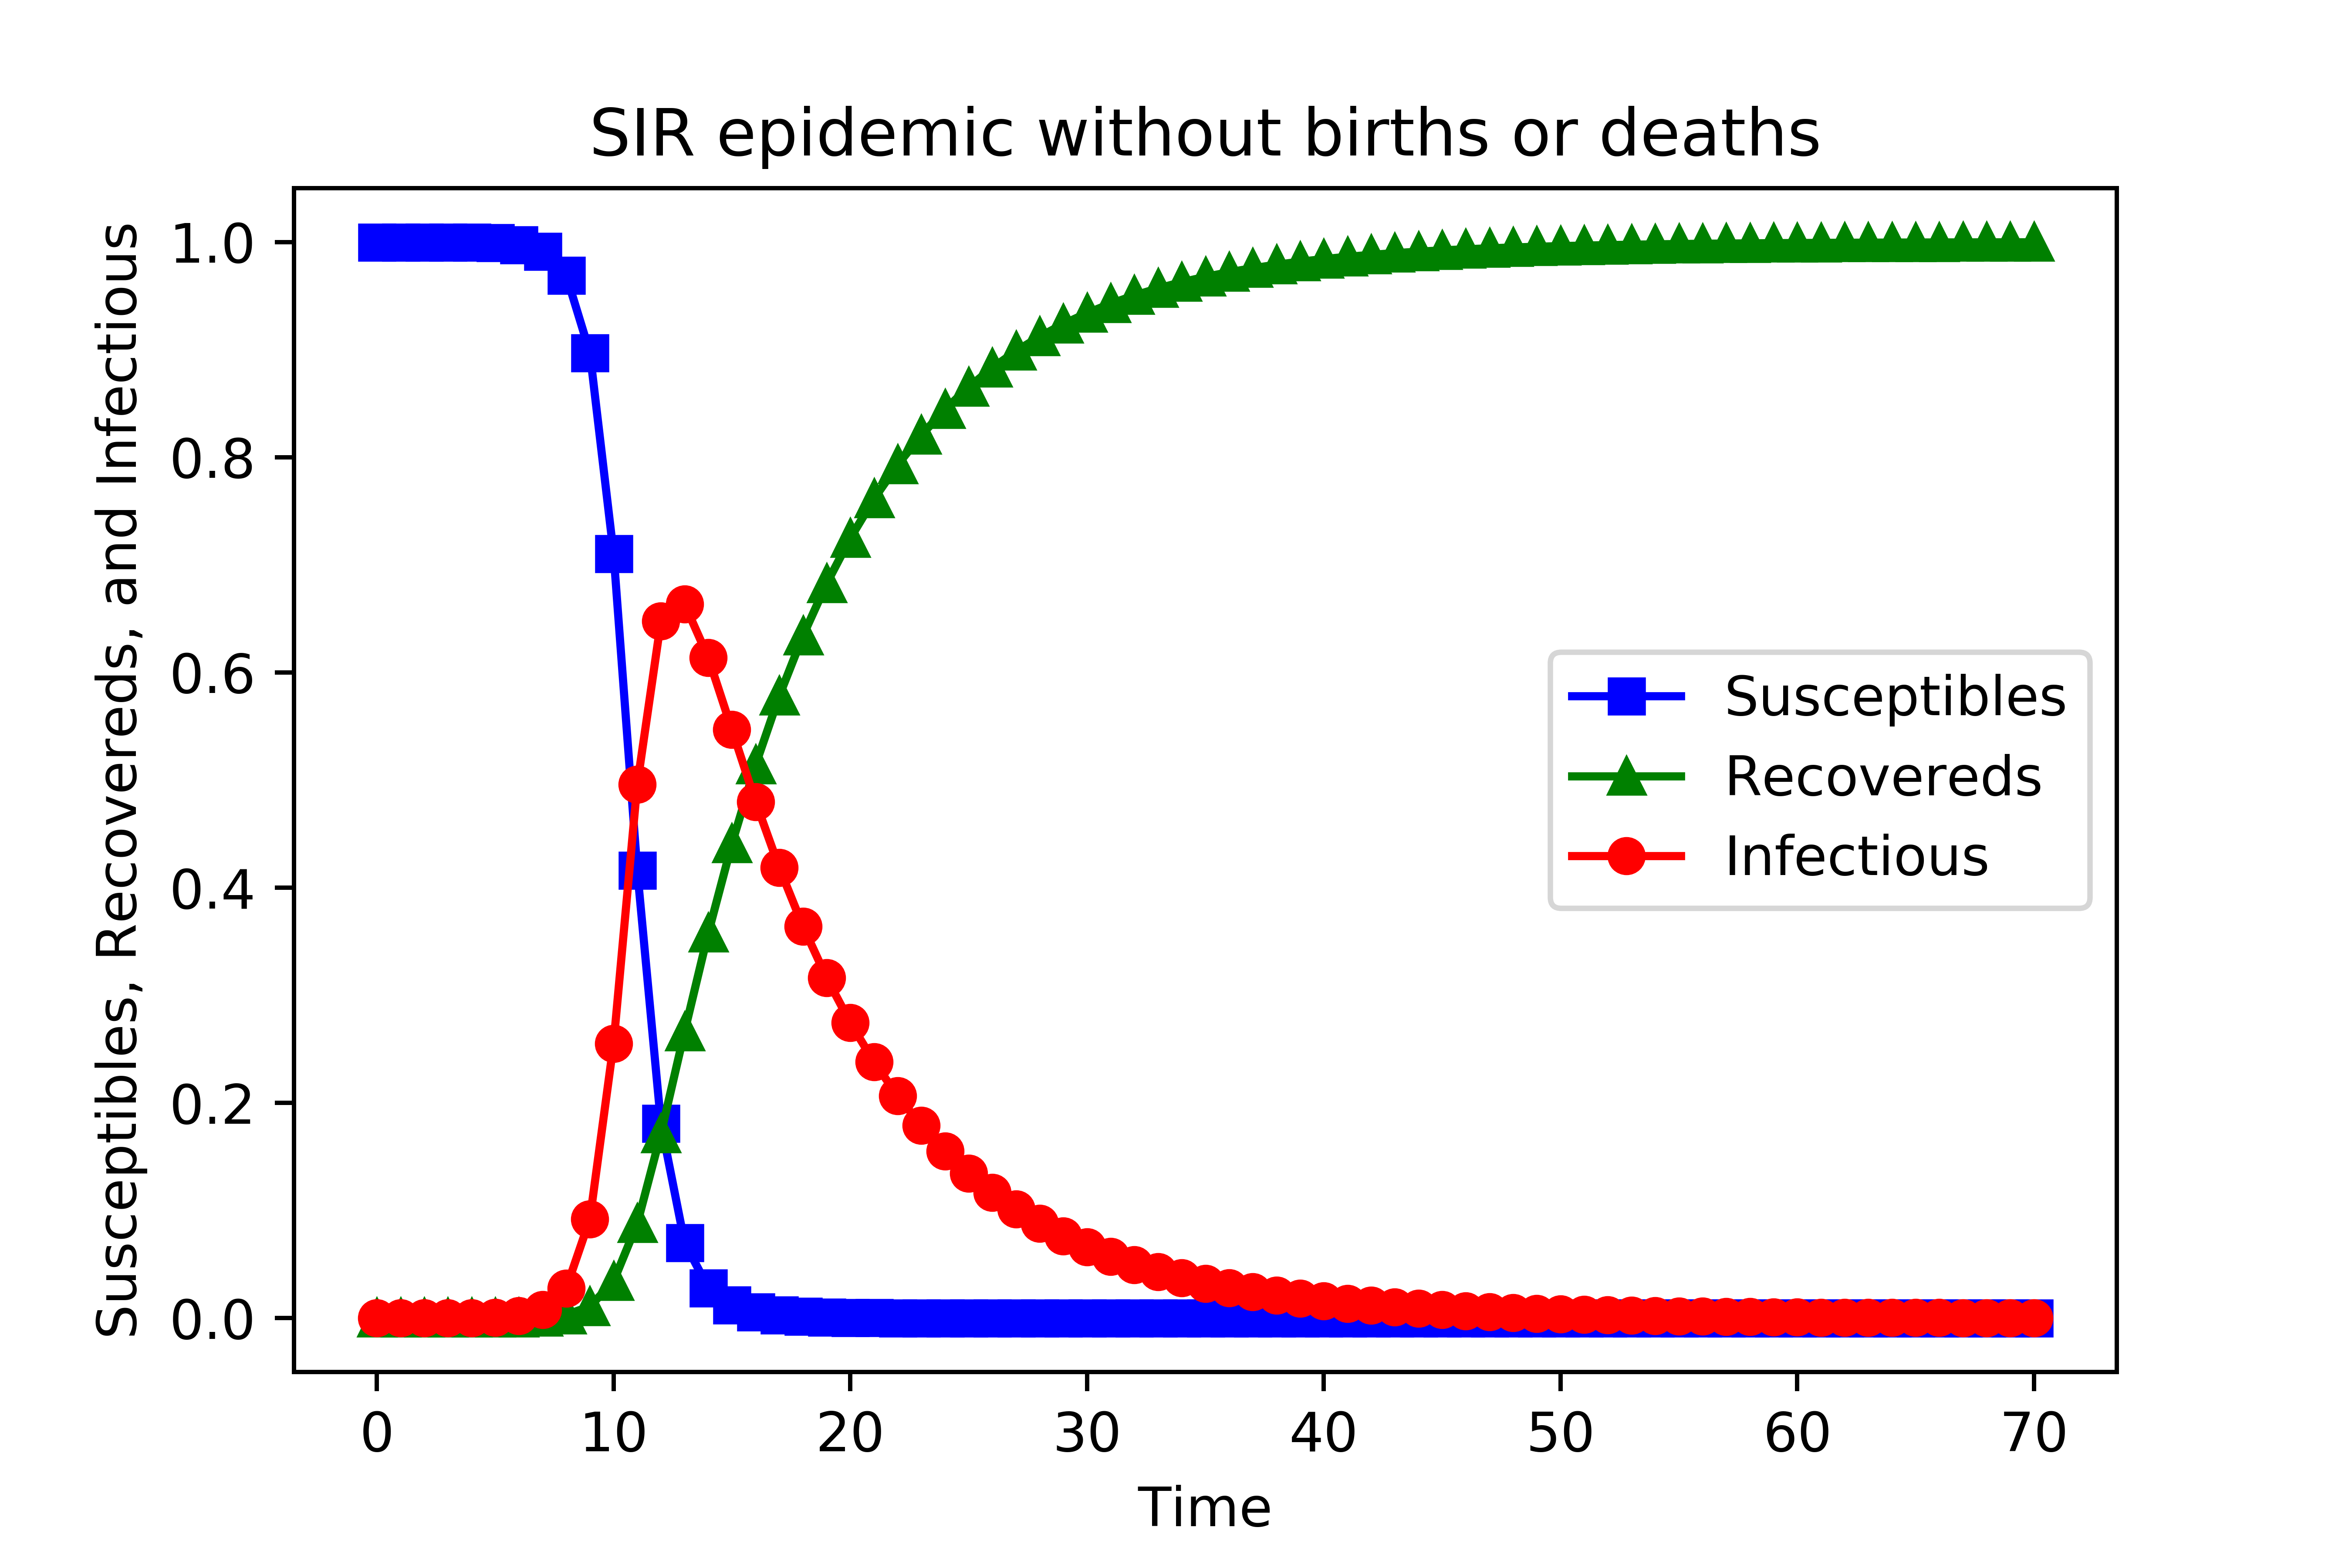
\includegraphics[width=0.8\textwidth]{img/SIR.png}
			\caption{SIR} 
			\label{img}
		\end{figure}	
		
		\section{变种的传染病模型}
		
		在二中讨论的三种模型具有理想的假设情况,有时并不符合实际情况,因此,会有研究对以上三种模型进行改进。建立传染病传播模型主要有三种方法第一种是单一群体方法,将人群看作一个整体,流行过程表现在易感者,感染者等各类人员数计量的变化。第二种是复合群体方法,考虑人群在空间上的异质性,将人群划分为多个子群体,各子群体之间因人员流动,形成复杂动态系统。第三种是微观个体方法,建模出发点是人群中的个体,个体有各自的属性和行为规则,个体之间形成接触网络,感染者和易感者的接触导致易感个体状态的变化。
		
		\subsection{单一群体模型}
		
		单一群体模型采用宏观视角建模,关注整个人群状态的变化,一般采用偏微分方程描述最流行的单一群体模型是仓室模型,所有处于相同状态的人构成一个仓室,随着状态的变化,人员在仓室之间移动仓室模型的基本假设是:每个人都相同;人群均匀混合;接触是瞬时的,接触与历史无关;每个仓室的人口数量足够大;在传染病流行过程中,感染率,恢复率是常数。
		\par\setlength\parindent{2em}SIR是经典的仓室模型。在SIR模型的基础上,仓室模型主要在以下几个方面进行了扩展:一是采用不同的仓室设置;二是考虑人口动力学,特别是将人口年龄结构看作重要因素;三是考虑更多的因素,如随机性,人口,空间的异质性等。
		\begin{itemize}
			\item 1)仓室设置:仓室对应着传染病流行过程中的可能状态,仓室的划分首先与传染病特性有关。经典SIR模型适合治愈后获得终生免疫的疾病。某些疾病治愈后不能获得免疫力,则可用SIS模型。若康复后能够获得一定的免疫力,但免疫力会遂渐消失, 则可用SIRS模型。某些疾病有潜伏期暴露,则可用SEIR模型。某些疾病新生儿可从母亲获得被动免疫,但一段时间后免疫力消失,则可采用MSEIR模型对表示从母亲获得被动免疫的人群。与此类似, 还有许多仓室设置方式。
			\item 2)人口年龄结构:年龄也是影响传染病流行的重要因素,个体感染传播疾病的可能性往往与年龄有关, 疫苗接种计划往往也和年龄有关。很多研究者用年龄结构模型研究传染病流行问题。对年龄的处理方法有两种,一是采用连续年龄结构, 二是将人口划分为多个年龄组。引入人口年龄结构后,传染病模型比较复杂,分析求解难度大但这类模型更好的刻画了年龄异质性对传染病流行的影响, 在很多国家人口分龄数据容易获得, 因此年龄结构传染病模型得到了较多的应用。			
			\item 3)随机性:传染病流行过程包含很多随机因素。随机性模型几乎是和确定性模型同时发展出来的。将随机模型中的随机变量用其数学期望代替,可得到随机模型对应的确定性模型。在很多情况下,如果人口总量很大,则二者有基本相同的性质。但在一些情况下, 随机模型与确定性模型有质的不同。在传染病出现早期或即将消失时, 感染人数较少,随机性发挥明显的作用, 确定性模型不适用。另外, 某些反复出现的传染病,随机性也发挥重要作用。在这些情况下, 随机性模型所探讨的入侵门槛, 续存条件, 传染病消失时间等,比确定性模型更有效。		
			\item 4)异质性:传统的仓室模型采用同质性假设, 然而很多情况下人群具有差异性。为了考虑人群差异,往往将人群分为多个组,分组的依据多种多样,可以是传播途径,接触方式,潜伏期,感染期等,也可能是社会,经济,人口等因素。例如Lajmnaovich等对分为n组的SIS模型进行分析, 发现了门槛条件, 证明了无病均衡和地方病均衡的全局稳定性。
		\end{itemize}
		
		
		\subsection{复合群体模型}
		
		不同地区之间因人员移动导致传染病传播的现象非常普遍,理解人类移动模式对传染病流行的影响已经引起了广泛关注。来源于生态学的复合群体(也称为复合种群等)模型在传染病领域得到应用。复合群体是指一个相对独立地理区域内各局域种群的集合,各局域种群通过个体迁移而连为一体。在研究传染病传播时,复合群体模型将人群看作由定义明确的社会单元形成的空间结构化人口,各单元之间因个人移动产生联系。每个社会单元是一个子群体,所有社会单元形成复合群体。
		\par\setlength\parindent{2em}复合群体模型多种多样, 但有两个基本特征一是子群体之间的藕合方式, 二是子群体内部动态的表达。常见的子群体藕合方式有三类:一是全连接结构, 各子群体之间完全互联, 个体可以向其他任何子群体迁移;二是局部连接结构, 一般采用规则网格,个体只能向相邻子群体迁移;三是网络结构, 子群体之间的连接关系用网络描述, 个体只能向邻接子群体迁移。如图5
     \begin{figure}
			\centering
			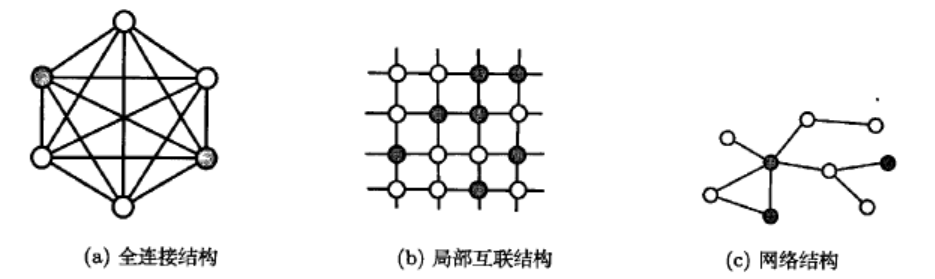
\includegraphics[width=0.8\textwidth]{img/ziqunti.png}
			\caption{子群体耦合} 
			\label{img}
		\end{figure}	
		\par\setlength\parindent{2em}由于复合群体模型考虑了子群体之间的迁移,研究传染病模型得到的结论更有现实意义。
		
		
		\subsection{微观个体模型}
		
		单一群体模型或复合群体模型的子群体中,一般假设个体同质,人群均匀混合。但实际上个体只能与有限个体接触,个体接触模式差异也较大,用网络描述接触模式更符合实际。大量研究表明网络结构对传染病动力学有显著影响, 如Keeling指出网络模型中平均接触数小以及高度集聚导致$r_0$减小, 传染病随机灭绝的概率小于均匀混合模型。对接触网络和个人行为模式的了解有助于建立更真实的传播模型。近几年基于网络的微观模型快速发展, 并在流感大流行干预措施研究中得到了成功应用。
		\par\setlength\parindent{2em}在传染病传播领域, 基于网络的微观个体模型目前有两个主要研究方向: 一是研究理想网络上的传染病传播,目的是揭示网络特性对传染病传播动力学的影响。部分原因是资源有限,很难获得精确的社会接触数据,并且了解网络特性与传染病传播的基本关系也很重要。二是研究现实网络上的传染病传播, 基本方法是进行实际调查,构造接近真实的接触网络, 在此基础上研究传染病传播。
		
		
		\section{总结}
		
		传染病是伴随人类发展的一个长期问题。通过建立传染病传播模型,可以从数学的角度,科学的研究传染病的传播,这对于理解传染病传播规律,预测传染病的发展趋势,评估应对措施等均具有积极的作用。在实际的研究中,我们应该根据实际的情况,选择合适的传播模型来对不同的传染病传播进行研究。
		
		
			
	\end{document}